% !TEX TS-program = lualatexmk
\documentclass[11pt]{article} 
\usepackage[margin=1in]{geometry} 
\usepackage[parfill]{parskip}% Begin paragraphs with an empty line rather than an indent
\usepackage{graphicx}
%\pdfmapfile{=Cochineal.map}
%\pdfmapfile{=newtx.map}
%\usepackage{amssymb}% don't use with newtxmath
%SetFonts
% cochineal+newtxmath
\usepackage[OT2,LGR,T2A,T1]{fontenc}
\usepackage{textcomp}
\usepackage[varqu,varl]{zi4}% inconsolata
\usepackage[p,osf,cochineal,vvarbb,amsthm]{newtx} % use proportional osf
\setmonofont{inconsolata}
%\usepackage{amsmath,amsthm}
%\usepackage[cochineal,vvarbb]{newtxmath}
% option vvarbb gives you stix blackboard bold
\usepackage[cal=boondoxo]{mathalfa}% less slanted than STIX cal
\usepackage{bm}
\usepackage{array,booktabs}
%SetFonts
\usepackage{fonttable}
\title{The Cochineal Font Package}
\author{Michael Sharpe}
\date{\today}  % Activate to display a given date or no date

\begin{document}
\maketitle
Cochineal is a fork of Crimson, a remarkable creation of Sebastian Kosch inspired by oldstyle font designers. The name Cochineal is intended to suggest that, while it is crimson, there may be bugs involved. More than 1500 glyphs were added to Crimson, allowing a more than modest chance that some poor spacing or kerning or accent placement might have been introduced. Such problems will occur in the less frequented parts of the fonts, and I would appreciate reports of problems you may discover. You are unlikely to trip over issues if you stay within the bounds of, say, the T$1$ encoding. I did correct problems in a number of glyphs from Crimson that FontForge uncovered and that could have led to poor rendition on some platforms, especially MAC OS. I also changed the emsize to {\tt 1000} (the standard for PostScript-flavored Opentype) from the Crimson value of {\tt  1024} and rescaled accordingly.

Cochineal provides {\tt Roman}, {\tt Bold}, {\tt Italic} and {\tt BoldItalic}. (Crimson provided semibold weights but with only limited coverage, which I did not wish to extend as this would have required the creation of about 2000 additional glyphs. Bob Tennent's {\tt Crimson} package does support semibold and the other styles, though  without my glyph additions.)

\textsc{Package Features:}\\
In addition to the encodings {\tt OT1}, {\tt T1}, {\tt TS1}, {\tt LY1} in general use by Western European (and some Eastern European) scripts, the package also offers {\tt LGR} with full support for monotonic, polytonic and some ancient Greek, and {\tt T2A} and {\tt OT2} Cyrillic support. All allow a choice from four figure styles---{\tt TLF} (tabular lining figures, monospaced and uppercase), {\tt LF} (proportional lining figures, uppercase), {\tt TOsF} (tabular oldstyle figures, monospaced and lowercase) and {\tt OsF} (proportional oldstyle figures, lowercase). The encodings {\tt OT1}, {\tt T1}, {\tt TS1}, {\tt LY1} offer \textsc{Small Caps}, even \textsc{\textit{Italics Small Caps}}, and additional figure styles---superiors, inferiors and denominators. These features are available from either \verb|fontspec| or from [pdf]\LaTeX. In \LaTeX, you access these through the macros \verb|\textsu|, \verb|\textinf| and  \verb|\textde|, or through their font-switching equivalents \verb|\sufigures|, \verb|\infigures| and  \verb|\defigures|. For example:
\begin{itemize}
\item
\verb|M\textsu{lle} Dupont| and \verb|M{\sufigures lle} Dupont| both produce M\textsu{lle} Dupont.
\item \verb|{\infigures 12345}| and \verb|\textinf{12345}| render as \textinf{12345}, dipping noticeably below the baseline,  while \verb|{\defigures 12345}| and \verb|\textde{12345}| render as \textde{12345}, aligned with the baseline.
\end{itemize}
As of version $1.062$ ($2020$), there is a new \verb|\textfrac| macro that works as in the following examples:
\begin{itemize}
\item
(two arguments) \verb|\textfrac{31}{32}| renders as \textfrac{31}{32};
\item
(three arguments) \verb|\textfrac[2]{63}{64}| renders as \textfrac[2]{63}{64}.
\end{itemize}
In addition, there is a \verb|\textcircled| macro that makes \verb|\textcircled{W}| render as \textcircled{W}. Numerals can also be circled: \verb|\textcircled{2}| renders as \textcircled{2}.

If you load the {\tt cochineal} package by means of option {\tt cochineal} to the {\tt newtx} package, version 1.71 or higher, there is a stacked fraction construction available using the macro \verb|\textsfrac| which behaves like \verb|\textfrac| except with the fractional part stacked vertically rather than diagonally. For example, \verb|\textsfrac[2]{5}{16}| produces \textsfrac[2]{5}{16}.

%\newpage
\textsc{Package Options and Macros:}\\
The package defines two macros, \verb|\useosf| and \verb|\useproportional|, useable only in the preamble, which determine the default figure style in text. A typical invocation would be something like
\begin{verbatim}
\usepackage{cochineal} % default figure style is tabular, lining
% load sans and typewriter fonts
% load a math font---it will use tabular lining figures in math
\useosf % switch from lining figures to oldstyle figures
\useproportional % switch from tabular to proportional
\end{verbatim}
There is a simpler way to achieve essentially the same result, but with the advantage that the figure styles are not loaded until after the math package (if any) is loaded, so that math always uses the default tabular lining figures. 
\begin{verbatim}
% If you use babel, load it here, before cochineal
\usepackage[p,osf]{cochineal} % default figure style is proportional, oldstyle
% load sans and typewriter fonts
% load a math font---it will use tabular lining figures in math
\end{verbatim}

As of version 1.71 of {\tt newtx}, it may be more convenient to use its mechanism for loading {\tt cochineal} as text and {\tt newtxmath} as math.
\begin{verbatim}
% If you use babel, load it here, before newtx
% load sans and typewriter fonts
\usepackage[p,osf,cochineal]{newtx} % text figure style is proportional, oldstyle, math will use tabular, lining figures
% if you use unicode latex with 
\end{verbatim}


No matter what the default figure style in text, the package provides switches and macros to use any available figure style.
\begin{itemize}
\item
\verb|\textlf{}| and \verb|{\lfstyle }| give proportional lining figures;
\verb|\texttlf{}| and \verb|{\tlfstyle }| give tabular lining figures;
\verb|\textosf{}| and \verb|{\osfstyle }| give proportional oldstyle figures;
\verb|\texttosf{}| and \verb|{\tosfstyle }| give tabular oldstyle figures;
\verb|\textfrac{3}{4}| uses superior and denominator figures to make the fraction \textfrac{3}{4}.
\end{itemize}
The options that can be passed to {\tt cochineal.sty} are the following:
\begin{itemize}
\item {\tt scale} or {\tt scaled}: a magnification factor---e.g., {\tt scaled=1.02} enlarges all text controlled by the package by {\tt2}\%;
\item
{\tt p}, or {\tt proportional}: make proportional figures the default rather than tabular;
{\tt lf}, or {\tt lining}: make lining figures the default (this is already the default);
{\tt osf}, or {\tt oldstyle}: make oldstyle figures the default rather than lining;
\item {\tt sups}: use superior figures to make footnote markers, rather than the \LaTeX's default markers;
\item {\tt swashQ}: use Cochineal's swash \Qswash\ instead of its tamer default version, \Qnoswash;
\item {\tt scosf}: always use oldstyle figures within a small caps block;
\item {\tt theoremfont}: for theorem statements in the {\tt plain} style, use a doctored version of italics that has upright figures, braces, brackets, parentheses, exclamation mark, colon and semicolon. It is implemented as the {\tt slanted} shape, and there are two options you can add to the call to the {\tt cochineal} package to modify the way it outputs figures.

The default (neither of the following options is set) is to use upright figures within theorem text, but in the same alignment (proportional or tabular) and the same style (lining or oldstyle) as in general text. 

Option {\tt thmtabular} causes figures in theorem text to render in tabular alignment, while option {\tt thmlining} causes figure styles to render in lining rather than oldstyle. The two may be used in conjunction, forcing figures  in theorem text to render as tabular lining figures.
\end{itemize}
\section*{Usage with unicode LaTeX}
The cochineal package works with all latex engines, and has some extra tricks available only in unicode LaTeX. In addition, {\tt newtx} also works with all latex engines and may be used to make a simplified call to use cochineal for text and {\tt newtxmath} (with cochineal letters) for math. Two crucial options---{\tt type1text} and {\tt nofontspec}---each of which may be used with both {\tt newtx} and {\tt cochineal}, determine how unicode latex will process your {\tt tex} document.
\begin{itemize}
\item
Neither {\tt type1text} (nor the equivalent {\tt type1}) nor {\tt nofontspec} specified: load {\tt fontspec} and use {\tt Cochineal} opentype fonts.
\item {\tt type1text} specified but not {\tt nofontspec}: load {\tt fontspec} but process text as {\tt pdflatex} would. (Other subsidiary opentype fonts could be loaded using {\tt fontspec} arguments.)
\item {\tt nofontspec} specified: {\tt fontspec} not loaded, text processed as under {\tt pdflatex}.
\end{itemize}
There are some more decorative glyph shapes as alternatives for Q and J in version 1.077 that are available only using unicode latex via {\tt StylisticSet=3} and {\tt StylisticSet=2} respectively. (The latter is available only in italic shapes.) They may be turned on as global options to {\tt newtx} or {\tt cochineal} by {\tt altQ}, {\tt altJ}.

\iftutex
\begin{verbatim}
\def\decorativeQ{{\addfontfeature{RawFeature=+ss03}Q}}
\def\decorativeJ{{\addfontfeature{RawFeature=+ss02}J}}
\end{verbatim}
\def\decorativeQ{{\addfontfeature{RawFeature=+ss03}Q}}
\def\decorativeJ{{\addfontfeature{RawFeature=+ss02}J}}
Q: \verb|\decorativeQ|: \decorativeQ\\
{\itshape J}:  \verb|\decorativeJ|: {\itshape \decorativeJ}\\
\fi
There is also an option {\tt oldSS} you may specify to use the older form of \verb|\SS| rather than the newer German Sharp S glyph.

\section*{Mathematical accompaniment}
The package contains fonts for use as math letters that are derived from Cochineal Roman and Greek glyphs and the {\tt newtxmath} family. Note that $v$ and $\nu$ (Greek {\tt nu}) are quite distinct. Here's a sample.

\begin{verbatim}
% preamble should include, in this order:
\usepackage[T1]{fontenc}
% load babel here
\usepackage[p,osf]{cochineal}
\usepackage[varqu,varl,var0]{inconsolata}
\usepackage[scale=.95,type1]{cabin}
\usepackage[cochineal,vvarbb]{newtxmath}
\usepackage[cal=boondoxo]{mathalfa}
\end{verbatim}
\def\Pr{\ensuremath{\mathbb{P}}}
\def\d{\mathrm{d}}
%\thispagestyle{empty}
The typeset math below follows the ISO recommendations that only variables
be set in italic. Note the use of upright shapes for $\d$, $\mathrm{e}$
and $\uppi$. (The first two are entered as \verb|\mathrm{d}| and
\verb|\mathrm{e}|, and in fonts derived from {\tt mtpro2} or {\tt newtxmath},
 the latter is entered as \verb|\uppi|.)

\textbf{Simplest form of the \textit{Central Limit Theorem}:} \textit{Let
$X_1$, $X_2,\cdots$ be a sequence of iid random variables with mean~$0$ 
and variance $1$ on a probability space $(\Omega,\mathcal{F},\Pr)$. Then}
\[\Pr\left(\frac{X_1+\cdots+X_n}{\sqrt{n}}\le v\right)\to\mathfrak{N}(v)\coloneq
\int_{-\infty}^v \frac{\mathrm{e}^{-t^2/2}}{\sqrt{2\uppi}}\,
\mathrm{d}t\quad\mbox{as $n\to\infty$, for every $v\in\mathbb{R}$,}\]
\textit{or, equivalently, letting} $S_n\coloneq\sum_1^n X_k$,
\[\mathbb{E} f\left(S_n/\sqrt{n}\right)\to \int_{-\infty}^\infty f(t)
\frac{\mathrm{e}^{-t^2/2}}{\sqrt{2\uppi}}\,\mathrm{d}t
\quad\mbox{as $n\to\infty$, for every $f\in\mathrm{b}
\mathcal{C}(\mathbb{R})$.}\]
\newpage

\section*{Cochineal's TS1 (textcomp)}
Coverage of TS1 has been enriched as of version $1.062$ so that it now qualifies as sub-encoding $0$, with essentially all TS1 features available.

\fonttable{Cochineal-Roman-ts1}
\newpage
 \section*{Typesetting Greek with LaTeX}
Cochineal offers a rather complete LGR-encoded glyph collection, lacking just a few ancient symbols.
\fonttable{Cochineal-Roman-tlf-lgr}

The LGR encoding defines a transcoding from Roman characters to Greek characters according to the following scheme:

\newpage
\[\begin{array}{m{7pt}m{7pt}m{7pt}m{7pt}m{7pt}m{7pt}m{7pt}m{7pt}m{7pt}m{7pt}m{7pt}m{7pt}m{7pt}m{7pt}m{7pt}m{7pt}m{7pt}m{7pt}m{7pt}m{7pt}m{7pt}m{7pt}m{7pt}m{7pt}m{7pt}m{7pt}}
A & B & C & D & E & F & G & H & I & J & K & L & M & N & O & P & Q & R & S & T & U & V & W & X & Y & Z  \\ 
\end{array}\]
\fontencoding{LGR}\selectfont
\[\begin{array}{m{7pt}m{7pt}m{7pt}m{7pt}m{7pt}m{7pt}m{7pt}m{7pt}m{7pt}m{7pt}m{7pt}m{7pt}m{7pt}m{7pt}m{7pt}m{7pt}m{7pt}m{7pt}m{7pt}m{7pt}m{7pt}m{7pt}m{7pt}m{7pt}m{7pt}m{7pt}}
A & B & C & D & E & F & G & H & I & J & K & L & M & N & O & P & Q & R & S & T & U & V & W & X & Y & Z  \\  
    a & b & c & d & e & f & g & h & i & j & k & l & m & n & o & p & q & r & sv & t & u & v & w & x & y & z \\ 
\end{array}\]
\fontencoding{T1}\selectfont

The file {\tt lgrenc.def}, which is loaded whenever {\tt LGR} is first loaded, specifies the above and more transcodings from Latin to Greek. See the {\tt usage.pdf} file in the {\tt babel-greek} documentation. 

The {\tt tfm} files associated with the Cochineal {\tt LGR } encoding were constructed with ligatures defined so that most Greek characters could be constructed using Latin input.

Note that you do not have to load the {\tt babel} package in order for the transcoding and ligatures to function properly.
%\newpage
\section*{Using Cochineal LGR Greek in other LaTeX packages}
There is nothing particular about Cochineal here that would not apply to any other text font package with a working LGR setup, as described above. There was for a number of years a small package {\tt substitutefont} that allowed the substitution of, say, LGR Cochineal Greek as the LGR Greek font in another text font package that lacked a suitable one of its own. This functioned less well as LaTeX evolved and its functionality was absorbed in 2020 sby the LaTeX command \verb|\DeclareFontFamilySubstitution|, which shares some of the problems of the now obsolete \verb|\substitutefont|. I've added this short section to describe some work-arounds those who wish to have access to this functionality.

Here are the problems I encountered:
\begin{itemize}
\item
If you try to add LGR Cochineal Greek to another package that has no support for LGR Greek, the attempt would fail. The work-around is to add in your preamble lines like
\begin{verbatim}
\usepackage[LGR,T1]{fontenc}
\DeclareFontFamily{LGR}{\rmdefault}{}
\end{verbatim}
after loading the text font package.
\item
Many text font packages do not settle on the final definition of \verb|\rmdefault| until just  before processing \verb|\begin{document}|. You may take care of all possibilities by adding to your preamble (near the end), imagining we are adding Cochineal LGR Greek to newtx:
\begin{verbatim}
\DeclareFontFamilySubstitution{LGR}{ntxtlf}{Cochineal-TLF}
\DeclareFontFamilySubstitution{LGR}{ntxlf}{Cochineal-LF}
\DeclareFontFamilySubstitution{LGR}{ntxtosf}{Cochineal-TOsF}
\DeclareFontFamilySubstitution{LGR}{ntxosf}{Cochineal-OsF}
\end{verbatim}
To reconcile the difference in size between {\tt newtx} and {\tt Cochineal}, with respective x-heights of 450 and 432, the former is 1.042 times taller than the latter, and so we have to set the scale for Cochineal, \verb|\Cochineal@scale| to 1.042 times that of newtx, \verb|\ntx@scale|. So, the next line in the preamble should be something like
\begin{verbatim}
\makeatletter
\@tmpdima=\ntx@scale\p@ \@tmpdima=1.042\@tmpdima
\def\Cochineal@scale{\strip@pt\@tmpdima}
\makeatother
\end{verbatim}
\end{itemize}

 \section*{Typesetting Russian}
With T$2$A encoding, the process is the same as with other T$2$A-encoded fonts, though the gaps in coverage may affect users of a number of non-Russian Cyrillic scripts. The only figure style provided is tabular lining (TLF.)
%\newpage
\fonttable{Cochineal-Roman-tlf-t2a}

The OT$2$ encoding (supposedly obsolete, but still useful) is intended for limited use in producing Russian characters with a Western keyboard, making by means of \TeX\ a transliteration of ASCII for most characters in the range 33--122, and providing ligatures to generate the rest, just as in the Greek case. See the documentation of {\tt nimbus15} for further details.
%\newpage
\fonttable{Cochineal-Roman-tlf-ot2}
%\end{document}
%\newpage
\section*{Additional glyphs for use in German orthography}
Prior to version {\tt1.050}, {\tt cochineal} offered basic support for German orthography, having all required accented glyphs and the lower case \ss, as well as a small caps \textsc{\ss}. Under LaTeX, the T$1$ encoding contained \verb|S_S|, but only as a synthesized character in the {\tt tfm}. Unicode users could not make use of \verb|S_S| as it was not present in the~{\tt otf}. So, with unicode tex processing:
\begin{verbatim}
{\addfontfeature{StylisticSet=1}\ss\ \textsc{\ss}}
\end{verbatim}
typesets, as in LaTeX processing, to

\ss\ \textsc{\ss}

Note also that in unicode processing, in order to obtain the expected case change behavior, it may be necessary to add in your preamble:
\begin{verbatim}
\uccode`ß="1E9E
\end{verbatim}


 As of version {\tt1.050} of {\tt cochineal}, there are now glyphs in each style for {\tt U+1E9E} and for its small caps version, as well as \verb|S_S| as a real character, accessible under unicode TeX. The glyphs may be used as the uppercase and small caps versions of {\tt germandbls}. Currently, the new glyphs are not available in any of the LaTeX encodings and must be used via unicode TeX.

The following tables show how to access the new glyphs in unicode TeX. Note that you will need to set {\tt StylisticSet=1} if you wish not to use the new sharp-s glyphs.

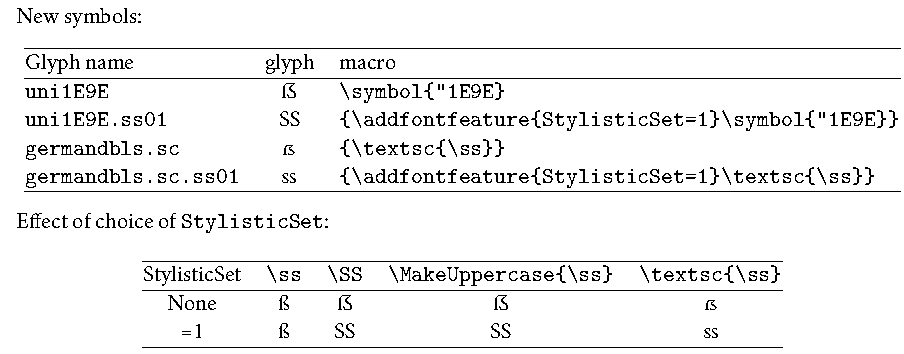
\includegraphics{newgermanglyphs-crop}
\end{document}  